% !TeX spellcheck = sk
\documentclass{article}

\usepackage{tikz}
\usetikzlibrary{arrows}
\usepackage{verbatim}
\usepackage{xcolor}
\usepackage{listings}
\usepackage{graphicx}
\usepackage[slovak]{babel}
\usepackage[latin2,utf8x]{inputenc}

\lstdefinestyle{BashInputStyle}{
  language=bash,
  basicstyle=\small\sffamily,
  numbers=left,
  numberstyle=\tiny,
  numbersep=3pt,
  frame=tb,
  columns=fullflexible,
  backgroundcolor=\color{yellow!20},
  linewidth=0.9\linewidth,
  xleftmargin=0.1\linewidth
}

\title{Užívateľská príručka pre SimArm}
\date{December 06 2016}
\author{Juraj Fojtí­k}
\begin{document}
\maketitle
\section{Stromový diagram:}
\tikzstyle{int}=[draw, fill=blue!20, minimum size=2em]
\tikzstyle{init} = [pin edge={to-,thin,black}]
\begin{tikzpicture}[node distance=2.5cm,auto,>=latex']
    \node [int] (s) {Server};
    \node [int] (3) [below of=s] {Klient 3};
    \node [int] (2) [left of=3] {Klient 2};
    \node [int] (1) [left of=2] {Klient 1};
    \node [int] (4) [right of=3] {Klient 4};
    \node [int] (5) [right of=4] {Klient 5};
    \path[<->] (s) edge node {} (1);
    \path[<->] (s) edge node {} (2);
    \path[<->] (s) edge node {} (3);
    \path[<->] (s) edge node {} (4);
    \path[<->] (s) edge node {} (5);
\end{tikzpicture}\newline\newline
Server: prenos dát medzi klientami\newline
Klient1: Riadenie prvého motora(v čase)\newline
Klient2: Riadenie druhého motora(v čase)\newline
Klient3: Nastavovanie základných parametrov robotickej ruky(užívateľské rozhranie)\newline
Klient4: Prepočet pozícií pre grafické zobrazenie robotickej ruky\newline
Klient5: Zobrazenie robotickej ruky v okne(užívateľské rozhranie) \newline\newline
Klienti určené pre užívateľské rozhranie s detailnejšie rozobraté v užívateľskom manuáli na str. 2,3
\section{Manuál inštalácie:}
\textbf{1. Inštalácia OpenCV:}
\begin{lstlisting}[style=BashInputStyle]
    $ chmod +x opencv2_4_6_1.sh 
    $ sudo ./opencv2_4_6_1.sh
\end{lstlisting}
\textbf{2. Kompilácia lokálnej a zdielanej knižnice pomocou nasledujúcich prí­kazov:}
\begin{lstlisting}[style=BashInputStyle]
    $ sudo make local_lib
    $ sudo make shared_lib
\end{lstlisting}
\textbf{3. Kompilácia serveru a jednotlivých klientov:}
\begin{lstlisting}[style=BashInputStyle]
    $ make   
\end{lstlisting}
\textbf{4. Spustenie serveru, a jednotlivých klientov(poradie otvorenia klientov nemá prioritu):}
\begin{lstlisting}[style=BashInputStyle]
    $ ./server 	-ilocalhost -p50000
    $ ./client1 -ilocalhost -p50000
    $ ./client2	-ilocalhost -p50000
    $ ./client3 -ilocalhost -p50000
    $ ./client4	-ilocalhost -p50000
    $ ./client5 -ilocalhost -p50000
\end{lstlisting}
Ak nezadáte vstupné argumenty, tak budú nastavený základne = ip adresa na localhost a port 50000.\newline
\section{Užívateľský manuál:}
\textbf{Klient 3:}
Pri spustení klienta 3 je možné vidieť nasledujúce okno podľa obr.1. Tento klient slúži na sledovanie aktuálnej odozvy systému a nastavovanie parametrov. \newline
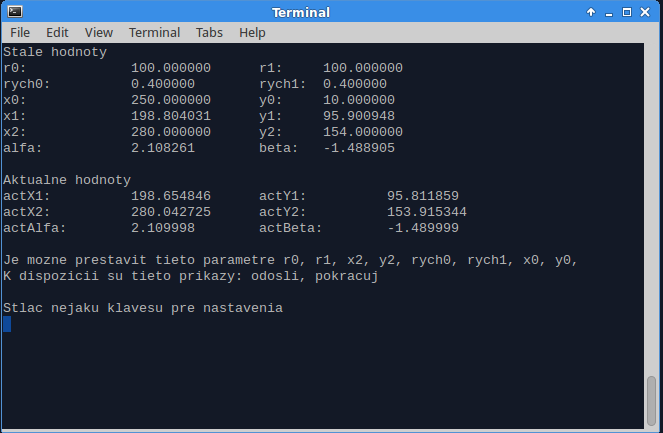
\includegraphics[width=\linewidth]{client3.png}
\begin{center} obr.1 \end{center}
Je tu možnosť nastaviť niekoľko parametrov ako:\newline
r0 = dĺžka ramena medzi prvým a druhým bodom robotickej ruky\newline
r1 = dĺžka ramena medzi druhým a tretím bodom robotickej ruky\newline
x0 = x-ová zložka počiatočného bodu\newline
y0 = y-ová zložka počiatočného bodu\newline
x2 = x-ová zložka koncového bodu\newline
y2 = y-ová zložka koncového bodu\newline
rych0 = rýchlosť posuvu motora1[rad/s]\newline
rych1 = rýchlosť posuvu motora2[rad/s]\newline
Nastavovanie sa vyvolá jednoduchým stlačením hociktorej klávesy a napísaním parametru, ktorý sa požaduje zmeniť. Následne sa potvrdí stlačením enteru, vloží sa hodnota na ktorá sa má zmeniť a stlačí sa enter. Ak chcete meniť ďalšie parametre postup opakujete, ak nie napíšete príkaz 'odosli', ktorý odošle do ďalších klientov potrebné informácie a následne je možné vidieť interakciu systému.
\newline
\textbf{Klient5:} Na obr. 2 možno vidieť grafické zobrazenie, ktoré vytvára klient 5. Slúži na 2D simuláciu aktuálneho stavu robotickej ruky a možnosť jednoduchého prestavenia koncového bodu kliknutím myši.\newline\newline
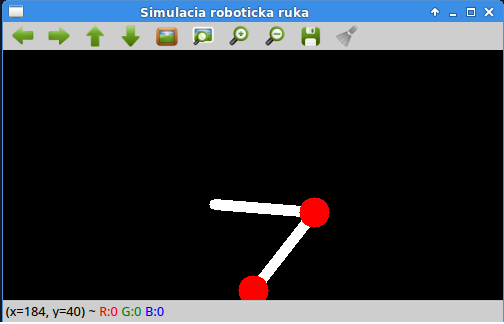
\includegraphics[width=\linewidth]{client5.png}
\begin{center} obr.2 \end{center}
\end{document}